\chapter{Stress Testing}
The purpose of the stress test is to observe how the system behaves as we steadily increase its load beyond the maximum number of users defined in the key performance scenarios. 

\section{Measurements}
We are interested to know whether the system will crash or if there will be a steady decline in response times. We are also interested in how the system recovers from an unusually high load; can the response times observed in our initial normal load test be replicated after the stress test without restarting the system? To answer these questions we measure throughput and average response times. We also measure errors and HTTP response codes.

\section{Test Setup}

\subsection{Increase Load}
To simulate stress on the system we created a series of tests which steadily increase the load on the server. We used the same mix of transactions used for load testing. The following set of tests were carried out for each the configs.


\begin{center}
\begin{tabular}{| c | c | c | c |}
\hline
Virtual Clients & Ramp up & Duration & Cool Down \\
\hline
20 & 300 & 300 & 60 \\ 
50 & 300 & 300 & 60 \\ 
80 & 300 & 300 & 60 \\ 
100 & 300 & 300 & 60 \\ 
150 & 300 & 300 & 60 \\
200 & 300 & 300 & 60 \\ 
300 & 300 & 300 & 60 \\ 
400 & 300 & 300 & 60 \\ 
. &  &  & \\ 
. &  &  & \\ 
2000 & 300 & 300 & 60 \\ 
\hline
\end{tabular}
\end{center}

The Jboss server was restarted only at the beginning of each series and not in between each test as had been the case with the load tests.


\subsection{Recovery}
In order to see how the system recovers we compare the results of our standard load test with a normal amount of users as defined in the key performance scenarios against the same test carried out after the system has experienced an exceptional high load.

\begin{center}
\begin{tabular}{| c | c | c | c |}
\hline
Virtual Clients & Ramp up & Duration & Cool Down \\
\hline 
2000 & 300 & 300 & 60 \\ 
500 & 300 & 600 & 60 \\ 
\hline
\end{tabular}
\end{center}

\section{Results}


\subsection*{Throughput} 
The throughput for the overall test is measured to determine the number of transactions the application can complete within each given time.


\begin{figure}[h]
\centering
\scalebox{0.65}{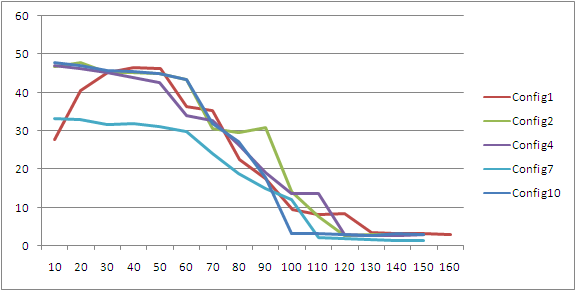
\includegraphics{Graphics/StressThroughput.png}}
\caption{Throughput under stress}
\label{fig:5.1}
\end{figure}

From the throughput test we see that after the maximum work rate is reached the system slowly declines as the load increases. At a certain point the decline stops and the steady state remains until a point when the server starts to refuse connections. 


\subsection*{Average Response Times} 
Generally, as the page sizes are very small and the response is delivered in one HTTP packet, the time to last byte and the time to first byte will be equal.

\begin{figure}[h]
\centering
\scalebox{0.65}{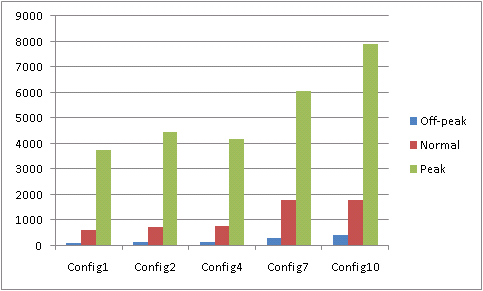
\includegraphics{Graphics/ResponseTimes2.png}}
\caption{Response Times - Time to Last Byte in Milliseconds}
\label{fig:5.3}
\end{figure}

The average response time slowly declines as the load increases. At a certain point the decline stops and the steady state remains as the server starts to refuse connections.


\subsection*{Recovery} 

\begin{figure}[h]
\centering
\scalebox{0.65}{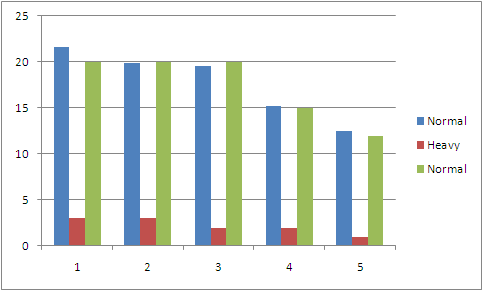
\includegraphics{Graphics/Recovery.png}}
\caption{System recovery from abnormal high load}
\label{fig:5.2}
\end{figure}

From these tests we observe that the systems ability to recover and continue to effectually service request at normal loads is not affected by the abnormally high load.


\subsection*{Errors} 
As the number of virtual clients is increased requests to the server are rejected. The following graph displays the percentage of rejected requests for each of the tests.

\begin{figure}[h]
\centering
\scalebox{0.65}{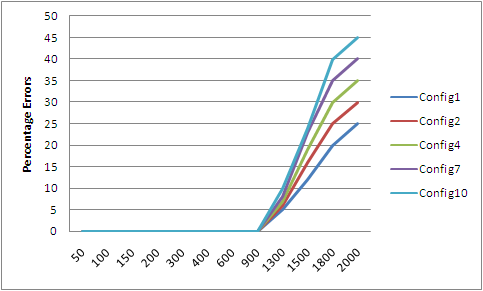
\includegraphics{Graphics/PercentageErrors.png}}
\caption{Percentage of responses containing errors}
\label{fig:5.3}
\end{figure}

\subsection*{Resource usage} 
During the tests we make a number of spot checks on the system resources.  We obsevered that the CPU was at maximum utilization.  Memory and Network resources where not under strain.  There where a number of TCP packets dropped due to the maximum utilization of the TCP buffer. 

